\documentclass{standalone}
\usepackage{tikz}
\usepackage{pgfplots}
\usepackage{mhchem}
\usepackage{nono}
\begin{document}
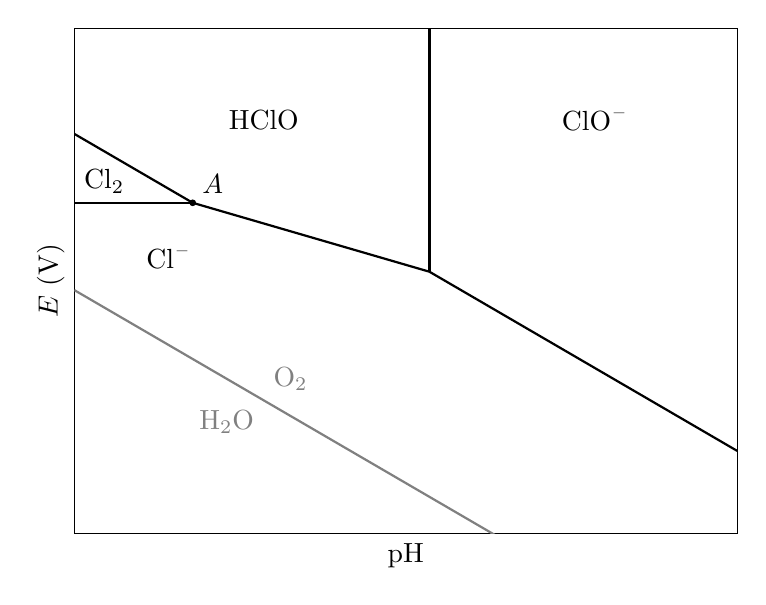
\begin{tikzpicture}
   \begin{axis}[
   ymax=1.8,
   xmin=0,
   xmax=14,
   ymin=0.7,
   height=8cm,
   width = 10cm,
   xlabel = pH,
   ylabel = $E$ (V),
   xtick=\empty,
   ytick=\empty,
   xticklabels={},
   yticklabels = {},
   ]
     \addplot[domain=0:2.5, thick] {1.42};
     \addplot[domain=0:2.5, thick] {1.57-0.06*x} coordinate (A);
     \addplot[domain=2.5:7.5, thick]{1.495-0.03*x};
     \addplot[domain=7.5:14, thick]{1.72-0.06*x};
     \addplot[domain=0:14, gray, thick]{1.23-0.06*x};
     \draw[thick] (axis cs:7.5, {1.495-0.03*7.5}) -- (axis cs:7.5, 2);
     \draw[fill] (A) circle(1pt) node[above right]{$A$};
     \draw (axis cs:2, 1.3) node{\ce{Cl-}};
     \draw (axis cs:4, 1.6) node{\ce{HClO}};
     \draw (axis cs:11, 1.6) node{\ce{ClO-}};
     \draw (axis cs:0, 1.42) node[above right]{\ce{Cl2}};
     \coordinate (B) at (axis cs:4, 1.23-0.06*4);
     \draw (B) node[above right, gray]{\ce{O2}};
     \draw (B) node[below left, gray]{\ce{H2O}};
   \end{axis} 
  \end{tikzpicture}
\end{document}
